% vim: spelllang=fr

\documentclass[../main.tex]{subfiles}
\graphicspath{{\subfix{../Figures/Chap1/}}}
\begin{document}

\begin{itshape}
Ce premier chapitre introduit les cyclones tropicaux (TC), de la simple définition jusqu'à la formulation de la question scientifique présentée dans cette thèse, en introduisant tous les concepts intermédiaires nécessaires.
\end{itshape}

\minitoc
%----------------------------------------------------------------------------
\section{Introduction aux cyclones tropicaux}

\subsection{Qu'est-ce qu'un cyclone tropical}

Du grec \textit{κύκλος}, nom commun désignant un cercle, ou plus généralement toute chose circulaire ou ronde, le terme cyclone, dans un contexte météorologique, fait référence au type de circulation atmosphérique dans lequel l'air se trouve en rotation atour d'un centre de basse pression. Sous cette définition, le terme de cyclone désigne une grande quantité d'objets aux caractéristiques très diverses et prenant place à différentes échelles spatiales et temporelles. Ainsi, à la
méso-échelle, ou échelle moyenne, caractérisée par des distances entre \SI{10}{\kilo\metre} et \SI{100}{\kilo\metre}, on peut notamment citer les mésocyclones, vortex d'air ascendant et convergeant, mesurant généralement moins de \SI{10}{\kilo\metre} de diamètre et observés dans les systèmes météorologiques convectifs, comme notamment les orages super-cellulaires. De l'autre côté du spectre, à l'échelle synoptique, c'est à dire à l'échelle traitant des distances de l'ordre du millier de kilomètres et sur des
temps caractéristiques de quelques jours, les plus grands objets météorologiques dépressionnaires pouvant être qualifiés de cyclones sont sans
nulle doute les vortex polaires ; de larges dépressions d'altitude situées près des pôles géographiques et dans lesquelles de l'air froid est en rotation. Malgré ces différences apparentes, tous les cyclones possèdent néanmoins des caractéristiques communes. Ainsi, le centre du cyclone est toujours l'endroit où la pression atmosphérique est la plus faible, et la circulation de l'air autour du centre est assurée à minima par l'équilibre entre la force induite par le gradient de pression radial d'une part, et la somme
de la force centrifuge ainsi que la force de Coriolis d'autre part -- équilibre qualifié de cyclostrophique. La force de Coriolis, force inertielle causée par la rotation de la Terre, est également la raison pour laquelle les cyclones tournent dans le sens contraire des aiguilles d'une montre dans l'hémisphère nord, et inversement dans l'hémisphère sud.

Les cyclones tropicaux -- que l'on abrègera ensuite par l'acronyme TC, selon l'appellation anglaise \textit{Tropical Cyclone} -- sont donc des phénomènes tourbillonnaires pouvant atteindre plusieurs centaines de kilomètres, les plaçant ainsi à la lisière entre la mésoéchelle et l'échelle synoptique. Ces objets prennent naissance, comme leur nom l'indique, dans la ceinture tropicale, définie comme la zone située entre le Tropique du Cancer dans l'hémisphère nord et le Tropique du Capricorne dans
l'hémisphère sud, et parfois approximée par la bande \ang{+20}~\ang{-20}~N. Les TCs se caractérisent par des vents violents autour du cœur, appelé œil ainsi que des précipitations pouvant être très intenses et organisées par bandes au sein de la spirale cyclonique, et ont également la propriété de posséder un cœur chaud en haute troposphère, propriété qui les distingue des cyclones extra-tropicaux.

\begin{figure}[t]
    \centering
    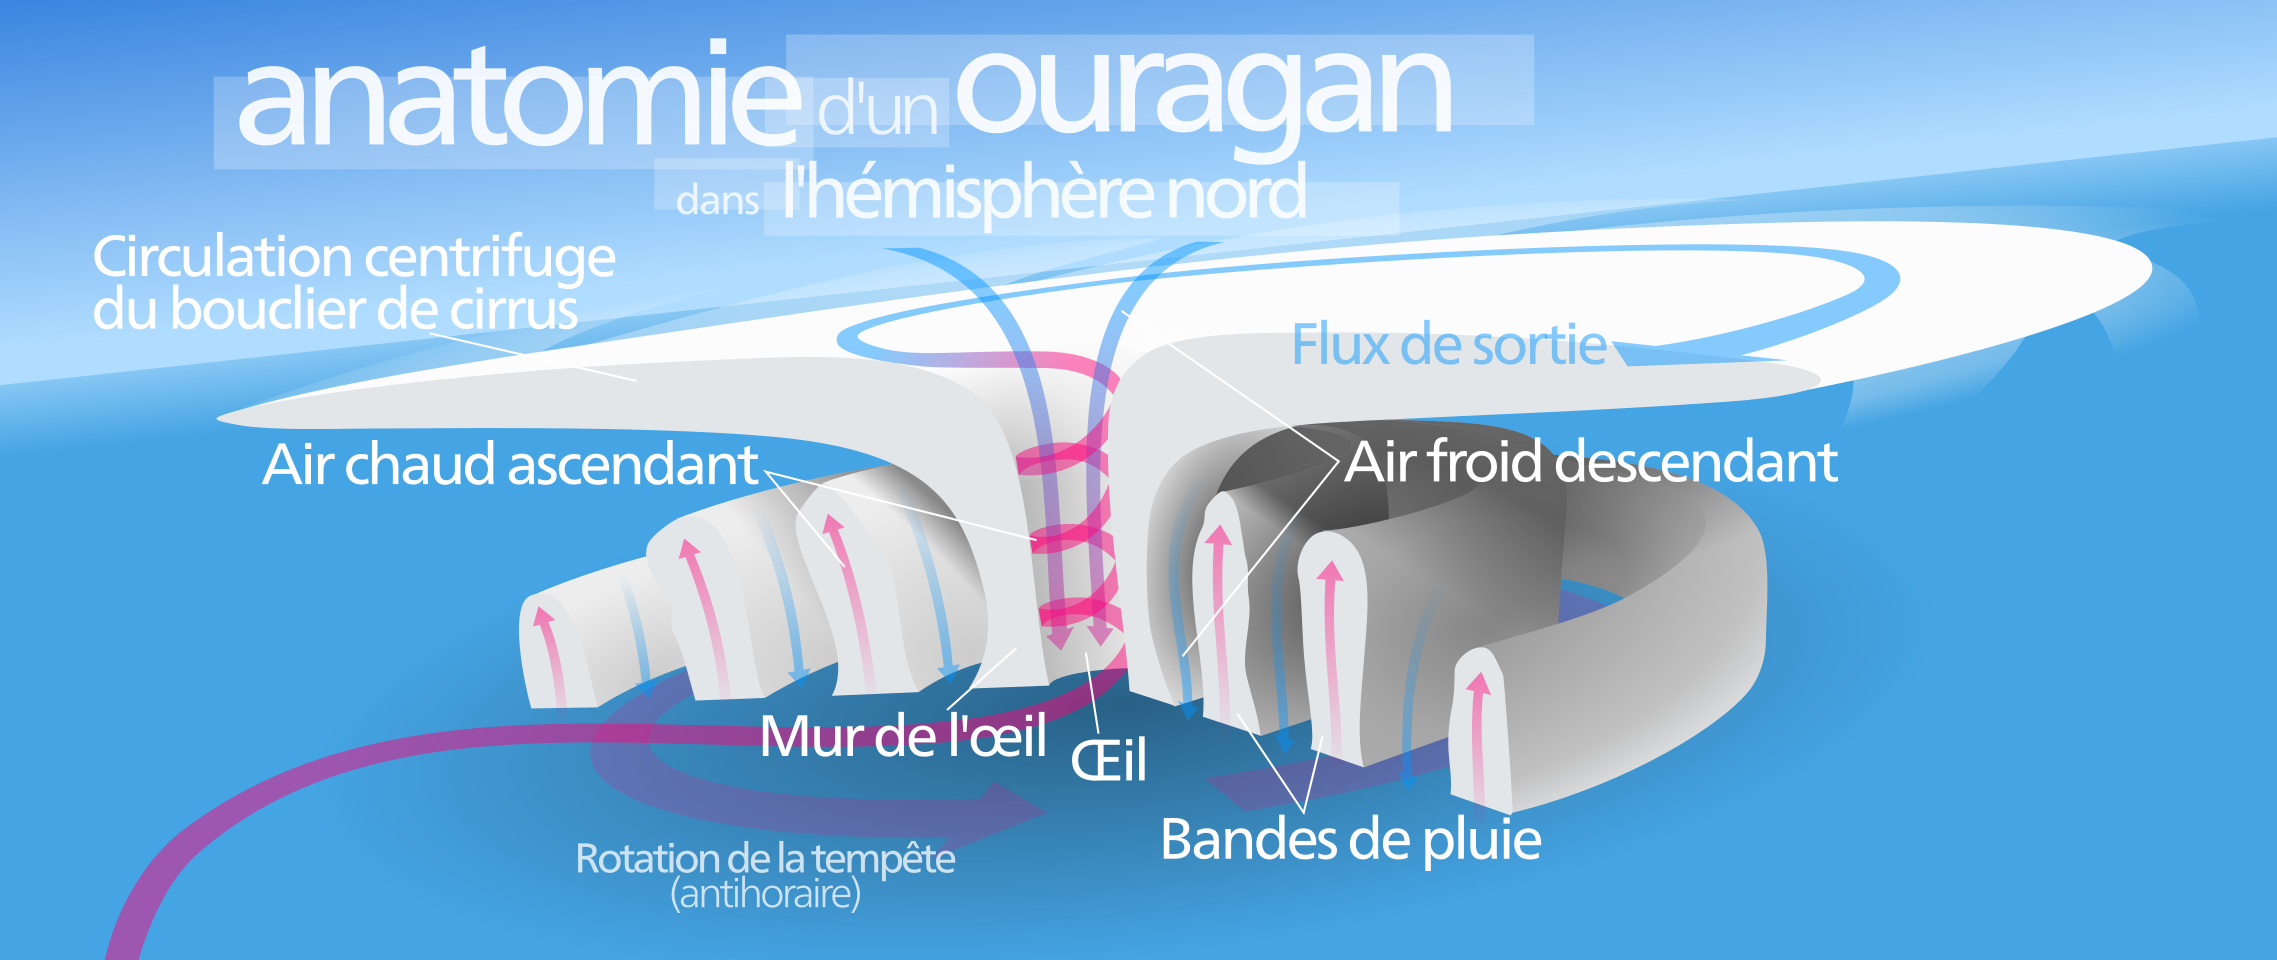
\includegraphics[width=0.9\textwidth]{Hurricane-fr.png}
    \caption{Diagramme en coupe d'un cyclone tropical, aussi appelé ouragan lorsqu'il survient dans l'océan Atlantique ou Nord-Est Pacifique -- By Kelvinsong - Own work, CC BY-SA 3.0, \url{https://commons.wikimedia.org/w/index.php?curid=23563610}}
    \label{fig:diagramme_TC}
\end{figure}

On dit que la perturbation dépressionnaire atteint le stade de cyclone tropical à proprement parler lorsque la vitesse du vent maximale à la surface et moyennée sur une certaine période, variable selon les régions du monde, atteint le seuil de \SI{33}{\metre\per\second}. En dessous de ce seuil, on parle soit de tempête tropicale si les vent sont supérieurs à \SI{17}{\metre\per\second} ou bien de dépression tropicale si le vent maximal y est inférieur.

\subsection{Bassins d'activité et saisonnalité}

À l'échelle planétaire, il y a entre \numrange[range-phrase ={ et }]{82}{85} TC par an en moyenne, à plus ou moins \num{8} TC près, selon les bases de données utilisées comme référence \parencite{schreck_impact_2014}. Cette activité globale est répartie sur un total de \num{6} grands bassins océaniques. Du point de vue opérationnel, c'est à dire pour ce qui traite des aspects de surveillance et de prévision de l'activité cyclonique, ces bassins océaniques peuvent en réalité être découpés
en sous régions, dans lesquelles un centre météorologique régional spécialisé (CMRS, ou RSMC en anglais) ou un centre d'avertissements de cyclones tropicaux (TCWC -- Tropical Cyclone Warning Centres) assure ces missions. Par exemple, l'océan Sud Indien est sous la tutelle conjointe, de part et d'autre du 90\textsuperscript{ème} méridien Est, du CMRS de l'île de la Réunion (Météo-France) pour toute la partie Ouest, incluant le canal du Mozambique, tandis que la surveillance de la partie Est est assurée par les TCWC de
Perth, rattaché au Bureau of Meteorology (BoM) Australien, et de Jakarta. Néanmoins, pour la régionalisation des analyses concernant l'activité cyclonique, nous favoriserons à travers ce document les grands bassins océaniques, et utiliserons des définitions des domaines adaptées des recommandations de \cite{knutson_tropical_2020}, proposées dans un effort de standardisation afin de faciliter la comparaison entre les études sur ce sujet. Ces bassins sont présentés sur la
\cref{fig:bassins_TC}.

\begin{figure}[t]
    \centering
    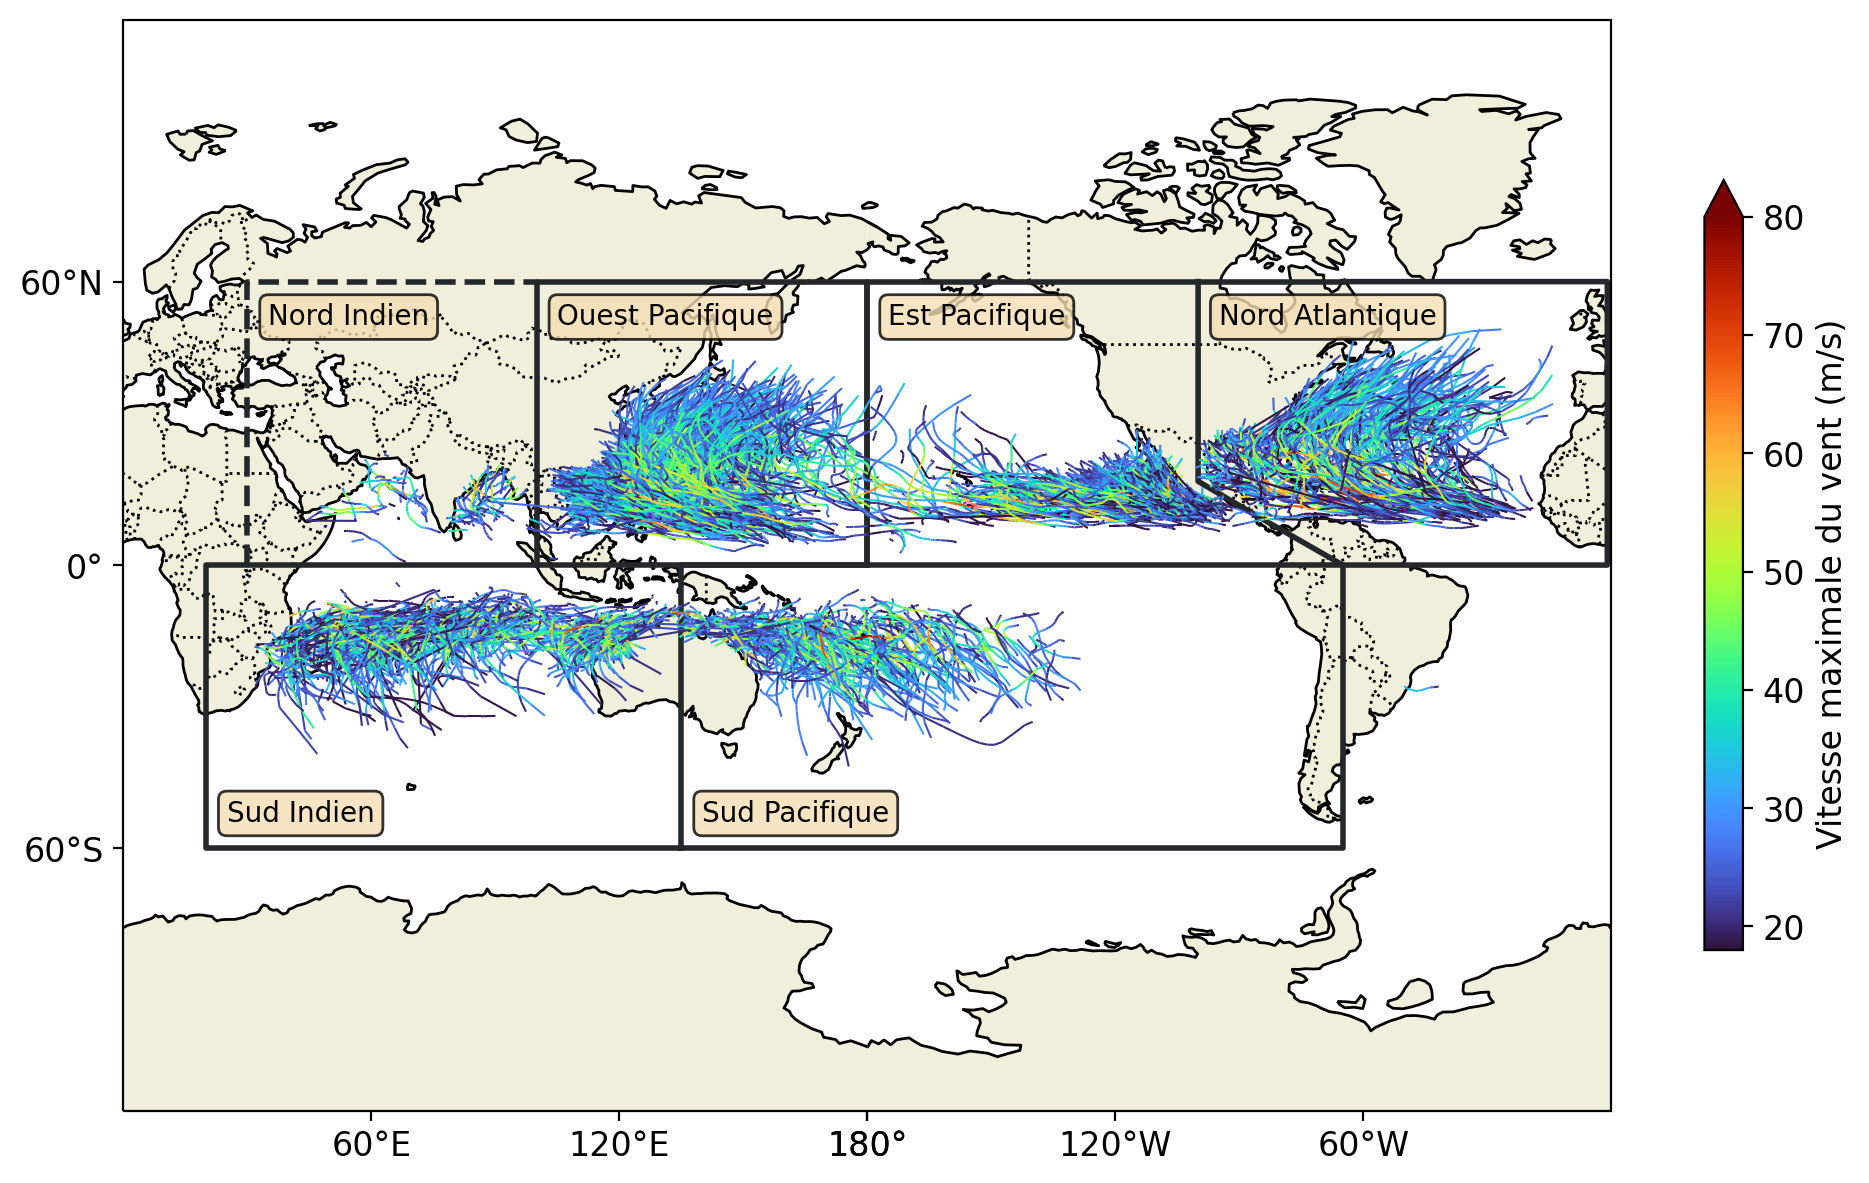
\includegraphics[width=0.9\textwidth]{Bassins_et_trajectoires.png}
    \caption{Bassins océaniques majeurs ainsi que les trajectoires des cyclones tropicaux observés entre 1981 et 2019, d'après la base de données \hbox{IBTrACS}. Les trajectoires sont colorées en fonction de l'intensité maximale des vents à chaque échéance. Les définitions des bassins océaniques utilisées ici, et plus généralement dans l'ensemble de ce document, sont issues, à quelques modifications près, des recommandations de \hbox{\cite[documents supplémentaires]{knutson_tropical_2020}}.}
    \label{fig:bassins_TC}
\end{figure}

Le bassin océanique concentrant la plus grande activité est le Ouest Pacifique.

\subsection{Risques associés et enjeux}

%-------------------------------------------------------------------------------
\section{Ingrédients de la cyclogénèse}
  
\subsection{Conditions de formation}

\subsection{Modèles conceptuels de fonctionnement}

\subsubsection{CISK}

\subsubsection{WISHE}

%-------------------------------------------------------------------------------
\section{Cyclones tropicaux et changement climatique}

\subsection{Bases de données observationelles}

\subsection{Les cyclones dans les modèles de climat}

\subsection{Consensus actuel sur les projections futures}

\subsection{Détection objective v.s indices de cyclogénèse}

%-------------------------------------------------------------------------------
\section{Synthèse}

\end{document}
